\section{信赖域模型}
\label{sec:tr-model}

既然局部模型只在一定范围内可靠，怎样把“只在这个范围内相信它”写成一个可以计算的问题？

\paragraph{贯穿全章的例子}
我们用下面这个二维目标：
\begin{equation}
 f(\bm{x})=\frac14x_1^4-\frac12x_1^2+x_1+\frac32x_2^2+x_2.
 \label{eq:tr-example}
\end{equation}
它的梯度和Hessian可以直接写出：
\begin{equation}
 \nabla f(\bm{x})=\begin{bmatrix}x_1^3-x_1+1\\3x_2+1\end{bmatrix},\qquad
 \nabla^2 f(\bm{x})=\begin{bmatrix}3x_1^2-1&0\\0&3\end{bmatrix}.
 \label{eq:tr-example-derivatives}
\end{equation}

令梯度为零，第二个分量给出$x_2=-1/3$，第一个分量是三次方程$x_1^3-x_1+1=0$，它只有一个实根$x_1\approx-1.3247$。这个驻点处Hessian正定，$f$又随$\lVert\bm{x}\rVert_2\to\infty$趋于正无穷，所以它就是全局最小点：
\[
 \bm{x}^\star\approx(-1.3247,\,-0.3333)^\top,\qquad f^\star\approx-1.5989.
\]

全章反复用到两个点。一个是$\bm{a}=(2,2)^\top$，这里Hessian正定，数据是
\begin{equation}
 f(\bm{a})=12,\qquad \bm{g}=\begin{bmatrix}7\\7\end{bmatrix},\qquad \bm{B}=\begin{bmatrix}11&0\\0&3\end{bmatrix}.
 \label{eq:tr-data-a}
\end{equation}
另一个是原点，这里Hessian不定，数据是
\begin{equation}
 f(\bm{0})=0,\qquad \bm{g}=\begin{bmatrix}1\\1\end{bmatrix},\qquad \bm{B}=\begin{bmatrix}-1&0\\0&3\end{bmatrix}.
 \label{eq:tr-data-o}
\end{equation}

\paragraph{模型能信多远}
在当前点$\bm{x}^{(t)}$展开到二阶，用位移$\bm{p}$作自变量，就得到\term{二次模型}（quadratic model）：
\begin{equation}
 m^{(t)}(\bm{p})=f(\bm{x}^{(t)})+\langle\bm{g}^{(t)},\bm{p}\rangle+\frac12\bm{p}^\top\bm{B}^{(t)}\bm{p}.
 \label{eq:tr-model}
\end{equation}
其中$\bm{g}^{(t)}=\nabla f(\bm{x}^{(t)})$，$\bm{B}^{(t)}$是对称矩阵，可以取Hessian $\bm{H}^{(t)}$，也可以取第~\ref{chap:quasi-newton}章由梯度差构造的近似。本节取$\bm{B}^{(t)}=\bm{H}^{(t)}$。

模型与目标差多少？例中$x_2$部分本来就是二次的，没有误差；$x_1$部分由四次多项式的展开直接得到，当$\bm{B}$取Hessian时
\begin{equation}
 f(\bm{x}+\bm{p})-m(\bm{p})=x_1p_1^3+\frac14p_1^4.
 \label{eq:tr-example-error}
\end{equation}

误差随$\lvert p_1\rvert$的增大而迅速增大。$\lvert p_1\rvert$很小时，高阶项微不足道；$\lvert p_1\rvert$到了$2$，在原点误差就是$4$，已经超过这里函数值变化的量级。图~\ref{fig:tr-model-slice}沿$x_1$方向画出了这件事，浅蓝带表示模型大致可信的范围。

\begin{BookInlineFigure}
 \centering
 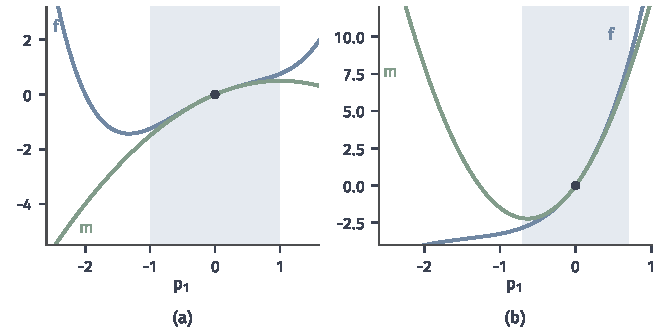
\includegraphics[width=112mm]{figures/05-optimization/02-smooth-optimization/matplotlib/tr-model-slice/figure.pdf}
 \caption{目标~\eqref{eq:tr-example}的$x_1$部分（蓝）与二次模型（绿）沿$p_1$的比较，黑点是展开点，浅蓝带是两者大致重合的范围。(a)~在$x_1=0$展开，曲率为负，模型向左无限下降，而目标很快转头向上。(b)~在$x_1=2$展开，曲率为正，模型有最小点，但左侧的目标比模型低得多。}
 \label{fig:tr-model-slice}
\end{BookInlineFigure}

图~\ref{fig:tr-model-contours}在平面上比较同一件事。在点$\bm{a}$附近，两组等高线几乎一样；离开圆盘之后，目标的等高线向左拉伸，模型仍是一组椭圆。

\begin{BookInlineFigure}
 \centering
 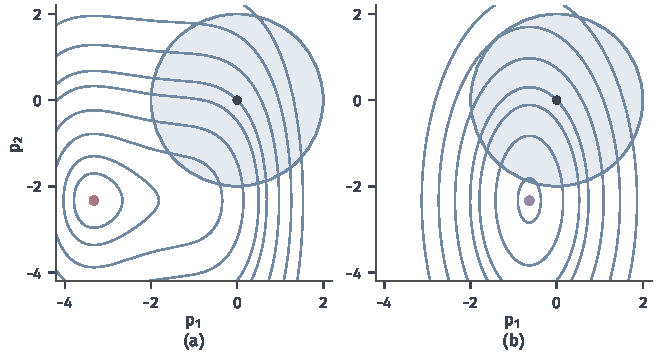
\includegraphics[width=112mm]{figures/05-optimization/02-smooth-optimization/matplotlib/tr-model-contours/figure.pdf}
 \caption{以$\bm{a}=(2,2)^\top$为原点的位移坐标下的等高线（蓝）。(a)~真实目标，红点是最小点。(b)~二次模型，紫点是模型的最小点。浅蓝圆盘半径为$2$，圆盘内两图相近，圆盘外差别明显。}
 \label{fig:tr-model-contours}
\end{BookInlineFigure}

\paragraph{子问题}
既然模型只在附近可靠，就只在附近找它的最小点。给定半径$\Delta^{(t)}>0$，定义\term{信赖域子问题}（trust-region subproblem）：
\begin{equation}
 \min_{\bm{p}\in\mathbb{R}^n}\ m^{(t)}(\bm{p})\qquad\text{满足}\quad\lVert\bm{p}\rVert_2\leq\Delta^{(t)}.
 \label{eq:tr-subproblem}
\end{equation}
半径$\Delta^{(t)}$约束的是这一轮的位移，原问题仍然是无约束的。下一轮换一个点、换一个半径，约束也跟着换。

半径的含义可以用一张手绘地图来理解。地图是在当前位置附近勘测的（对应二次模型），周围画得准，远处多半是推测。你决定只按地图走到某个距离为止（对应半径），走到后核对实地与地图是否相符，相符就下次敢走远些，不符就走近些（对应后面的半径更新）。这个类比有一处不贴切：半径并不是模型真实误差的边界，它只是算法根据最近的核对结果作出的估计，可能偏大，也可能偏小。

\paragraph{曲率不正定时}
第~\ref{chap:second-order-methods}章的Newton法要解$\bm{B}\bm{d}=-\bm{g}$。原点的数据~\eqref{eq:tr-data-o}上这个方程仍可解，解是
\[
 \bm{d}^{\mathrm{N}}=-\bm{B}^{-1}\bm{g}=\begin{bmatrix}1\\-1/3\end{bmatrix}.
\]

它与梯度的内积决定这个方向是上坡还是下坡：
\[
 \langle\bm{g},\bm{d}^{\mathrm{N}}\rangle=1-\frac13=\frac23>0.
\]
内积为正，这个方向是上坡方向。$\bm{d}^{\mathrm{N}}$只是模型的驻点，模型在这里是个鞍面。沿$\bm{d}^{\mathrm{N}}$作线搜索不会有任何下降的步长，所以线搜索框架不得不先修改$\bm{B}$，使它正定。

信赖域子问题没有这个麻烦。闭球是紧集，$m$连续，所以无论$\bm{B}$是否正定，最小点都存在。例中模型沿$p_1$轴是$p_1-p_1^2/2$，向左无限下降，无约束时没有最小点；加上半径之后，解就落在球的边界上。图~\ref{fig:tr-newton-ascent}画出了$\Delta=2$的情形：$\bm{B}$无需修改，负曲率反而被利用，它把解推向了边界。

\begin{BookInlineFigure}
 \centering
 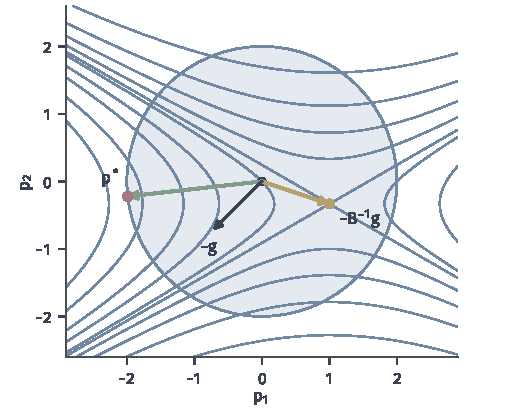
\includegraphics[width=88mm]{figures/05-optimization/02-smooth-optimization/matplotlib/tr-newton-ascent/figure.pdf}
 \caption{原点处的二次模型，蓝线是等高线，浅蓝圆盘半径$\Delta=2$。黄色箭头指向模型的驻点$-\bm{B}^{-1}\bm{g}$，黑色箭头是负梯度方向，红点是子问题的全局解$\bm{p}^\star$，绿色箭头指向它。黄色方向是上坡方向，而子问题的解利用负曲率走到了圆盘左侧边界。}
 \label{fig:tr-newton-ascent}
\end{BookInlineFigure}

\paragraph{与线搜索的对照}
第~\ref{chap:smooth-foundations}章的线搜索分两步：先选定下降方向$\bm{d}^{(t)}$，再沿这条射线选步长$\alpha^{(t)}$。信赖域把顺序倒过来：先选定半径，再同时决定方向和长度。半径变了，步的方向也跟着变。

在点$\bm{a}$，图~\ref{fig:tr-line-vs-region}画出了两者的差别。线搜索的候选点都在一条射线上；信赖域的解随半径变化走出一条曲线，半径小时贴近负梯度方向，半径大时转向Newton点。半径的调整因此比步长的调整多一层作用，它还在改变方向。

\begin{BookInlineFigure}
 \centering
 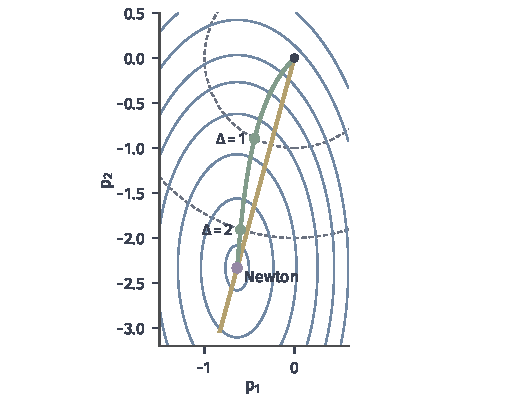
\includegraphics[width=86mm]{figures/05-optimization/02-smooth-optimization/matplotlib/tr-line-vs-region/figure.pdf}
 \caption{点$\bm{a}$处的二次模型等高线（蓝）。黄线是沿Newton方向的射线，线搜索只在这条线上选点。绿线是子问题的全局解随$\Delta$变化的轨迹，绿点是$\Delta=1$和$\Delta=2$时的解，虚线圆是对应的边界，紫点是Newton点。}
 \label{fig:tr-line-vs-region}
\end{BookInlineFigure}

表~\ref{tab:tr-vs-linesearch}把两种做法并列。

\begin{BookInlineTable}
 \centering
 \begin{tabular}{lll}
  \toprule
  & 线搜索 & 信赖域\\
  \midrule
  先固定的量 & 方向$\bm{d}^{(t)}$ & 半径$\Delta^{(t)}$\\
  后决定的量 & 步长$\alpha^{(t)}$ & 位移$\bm{p}^{(t)}$（方向和长度）\\
  $\bm{B}$的要求 & 需要给出下降方向 & 对称即可\\
  一次试探失败 & 缩短步长，方向不变 & 缩小半径，方向可变\\
  \bottomrule
 \end{tabular}
 \caption{线搜索与信赖域的分工对照。}
 \label{tab:tr-vs-linesearch}
\end{BookInlineTable}

\paragraph{子问题的全局解}
子问题虽然非凸，它的全局解却有干净的刻画。下面的定理说明，解满足一个被平移过的线性方程，平移量$\lambda$恰好使矩阵半正定。

\begin{theorem}[子问题的全局解]
 \label{thm:tr-exact}
 设$\bm{B}$对称，$\Delta>0$，$m$如式~\eqref{eq:tr-model}（省略上标$(t)$）。点$\bm{p}^\star$是子问题~\eqref{eq:tr-subproblem}的全局解，当且仅当$\lVert\bm{p}^\star\rVert_2\leq\Delta$，并且存在$\lambda\geq0$，使得
 \begin{equation}
  (\bm{B}+\lambda\bm{I})\bm{p}^\star=-\bm{g},\qquad
  \lambda(\Delta-\lVert\bm{p}^\star\rVert_2)=0,\qquad
  \bm{B}+\lambda\bm{I}\succeq\bm{0}.
  \label{eq:tr-exact-conditions}
 \end{equation}
\end{theorem}

\begin{proof}
 先证充分性。令
 \[
  \hat{m}(\bm{p})=m(\bm{p})+\frac{\lambda}{2}\lVert\bm{p}\rVert_2^2.
 \]
 它的Hessian是$\bm{B}+\lambda\bm{I}\succeq\bm{0}$，所以是凸函数；式~\eqref{eq:tr-exact-conditions}的第一式说明$\nabla\hat{m}(\bm{p}^\star)=\bm{0}$，因此$\bm{p}^\star$是$\hat{m}$的全局最小点。对任意$\lVert\bm{p}\rVert_2\leq\Delta$，把$\hat{m}(\bm{p})\geq\hat{m}(\bm{p}^\star)$展开，得到
 \[
  m(\bm{p})\geq m(\bm{p}^\star)+\frac{\lambda}{2}\bigl(\lVert\bm{p}^\star\rVert_2^2-\lVert\bm{p}\rVert_2^2\bigr).
 \]
 若$\lambda=0$，右端就是$m(\bm{p}^\star)$。若$\lambda>0$，第二式给出$\lVert\bm{p}^\star\rVert_2=\Delta$，括号非负。两种情形都有$m(\bm{p})\geq m(\bm{p}^\star)$。

 再证必要性。若$\lVert\bm{p}^\star\rVert_2<\Delta$，$\bm{p}^\star$是二次函数的内部局部极小点，于是梯度$\bm{B}\bm{p}^\star+\bm{g}=\bm{0}$，Hessian $\bm{B}\succeq\bm{0}$，取$\lambda=0$即可。

 下设$\lVert\bm{p}^\star\rVert_2=\Delta$，分三步。第一步找乘子。任取与$\bm{p}^\star$正交的单位向量$\bm{v}$，下面的曲线落在球面上：
 \[
  \bm{q}(\theta)=\cos\theta\,\bm{p}^\star+\Delta\sin\theta\,\bm{v}.
 \]
 $\theta=0$时函数$m(\bm{q}(\theta))$最小，导数为零：
 \[
  \Delta\,\langle\bm{B}\bm{p}^\star+\bm{g},\bm{v}\rangle=0.
 \]
 所以$\bm{B}\bm{p}^\star+\bm{g}$与所有切向量正交，它只能是$\bm{p}^\star$的倍数，记为$-\lambda\bm{p}^\star$，这就是第一式。

 第二步证$\lambda\geq0$。对$s\in[0,1]$，点$(1-s)\bm{p}^\star$可行，$m((1-s)\bm{p}^\star)$在$s=0$的右导数不能为负：
 \[
  -\langle\bm{B}\bm{p}^\star+\bm{g},\bm{p}^\star\rangle=\lambda\Delta^2\geq0.
 \]

 第三步证半正定。$\hat{m}$是二次函数且在$\bm{p}^\star$处梯度为零，所以
 \[
  \hat{m}(\bm{p})-\hat{m}(\bm{p}^\star)=\frac12(\bm{p}-\bm{p}^\star)^\top(\bm{B}+\lambda\bm{I})(\bm{p}-\bm{p}^\star).
 \]
 当$\lVert\bm{p}\rVert_2=\Delta$时，$\hat{m}$与$m$的差相同，而$m(\bm{p})\geq m(\bm{p}^\star)$，于是
 \[
  (\bm{p}-\bm{p}^\star)^\top(\bm{B}+\lambda\bm{I})(\bm{p}-\bm{p}^\star)\geq0.
 \]
 任取满足$\langle\bm{w},\bm{p}^\star\rangle\neq0$的$\bm{w}$，令
 \[
  \bm{p}=\bm{p}^\star-2\frac{\langle\bm{w},\bm{p}^\star\rangle}{\langle\bm{w},\bm{w}\rangle}\bm{w}.
 \]
 这是$\bm{p}^\star$关于$\bm{w}$的法平面的反射，长度仍为$\Delta$，而$\bm{p}-\bm{p}^\star$与$\bm{w}$平行，所以$\bm{w}^\top(\bm{B}+\lambda\bm{I})\bm{w}\geq0$。满足$\langle\bm{w},\bm{p}^\star\rangle\neq0$的$\bm{w}$在$\mathbb{R}^n$中稠密，由连续性，不等式对所有$\bm{w}$成立。
\end{proof}

三个条件各有作用。第一式说明解是一个被“加了$\lambda$”的Newton方程的解，$\lambda$越大，方程越接近$\lambda\bm{p}=-\bm{g}$，解越贴近负梯度方向。第二式说明半径不起作用时$\lambda=0$，解就是Newton点。第三式是全局性的来源：它要求$\lambda$至少抵消最负的特征值，只满足前两式的点可能只是局部解或驻点。

$\lambda$的作用类似预算约束下的影子价格：半径限得越紧，$\lambda$越大。这个类比只说明单调关系，$\lambda$的单位与目标值的单位并不相同。

\paragraph{怎样求$\lambda$}
设$\bm{B}$的特征值为$\lambda_1\leq\cdots\leq\lambda_n$，对应的单位正交特征向量为$\bm{q}_1,\ldots,\bm{q}_n$。当$\lambda>\max\{0,-\lambda_1\}$时，式~\eqref{eq:tr-exact-conditions}的第一式有唯一解$\bm{p}(\lambda)$，它的长度满足
\begin{equation}
 \lVert\bm{p}(\lambda)\rVert_2^2=\sum_{i=1}^n\frac{\langle\bm{q}_i,\bm{g}\rangle^2}{(\lambda_i+\lambda)^2}.
 \label{eq:tr-secular}
\end{equation}
每一项都随$\lambda$严格减小（只要系数不为零）。求解子问题于是化为一元方程$\lVert\bm{p}(\lambda)\rVert_2=\Delta$，称为\term{久期方程}（secular equation）。

点$\bm{a}$的数据~\eqref{eq:tr-data-a}上，取$\Delta=2$，式~\eqref{eq:tr-secular}成为
\[
 \lVert\bm{p}(\lambda)\rVert_2^2=\frac{49}{(11+\lambda)^2}+\frac{49}{(3+\lambda)^2}.
\]

$\lambda=0$时长度约为$2.419$，大于$\Delta$，Newton点在球外，所以$\lambda>0$。再试几个值：
\[
 \lVert\bm{p}(0.5)\rVert_2\approx2.091,\qquad
 \lVert\bm{p}(0.7)\rVert_2\approx1.984,\qquad
 \lVert\bm{p}(0.67)\rVert_2\approx1.9995.
\]

继续缩小区间，得到$\lambda\approx0.669$，相应的解是
\[
 \bm{p}^\star\approx(-0.600,\,-1.908)^\top.
\]
实际计算不用谱分解，而是对几个试探的$\lambda$作Cholesky分解，用Newton迭代解$1/\lVert\bm{p}(\lambda)\rVert_2=1/\Delta$；这个函数比长度本身更接近线性，几次迭代就够了。

图~\ref{fig:tr-secular}(a)是这条曲线。原点的数据上（图~\ref{fig:tr-secular}(b)），$\bm{B}$有负特征值$-1$，只能在$\lambda>1$的范围内找解。曲线在$\lambda=1$处趋于无穷，所以对任何半径都有交点，$\Delta=2$时$\lambda\approx1.503$。

\begin{BookInlineFigure}
 \centering
 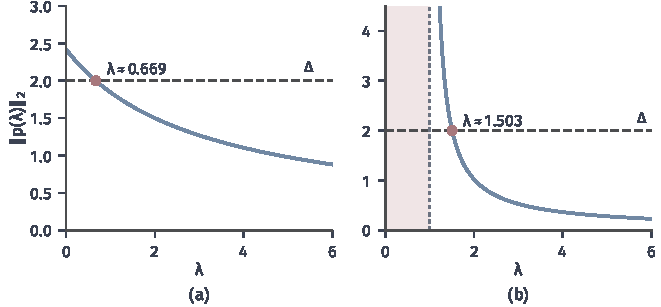
\includegraphics[width=112mm]{figures/05-optimization/02-smooth-optimization/matplotlib/tr-secular/figure.pdf}
 \caption{解的长度$\lVert\bm{p}(\lambda)\rVert_2$（蓝）与半径$\Delta=2$（虚线）的交点（红）给出乘子。(a)~点$\bm{a}$，$\bm{B}$正定，曲线从Newton步的长度开始下降。(b)~原点，$\bm{B}$的最小特征值为$-1$，红色浅底的区域$\lambda<1$不满足$\bm{B}+\lambda\bm{I}\succeq\bm{0}$。}
 \label{fig:tr-secular}
\end{BookInlineFigure}

\paragraph{困难情形}
上面的论证依赖$\langle\bm{q}_1,\bm{g}\rangle\neq0$。如果梯度与最小特征值的特征空间正交，式~\eqref{eq:tr-secular}中对应的项消失，曲线在$\lambda=-\lambda_1$处不再趋于无穷，久期方程可能无解。这称为子问题的\term{困难情形}（hard case）。

看下面这组数据：
\[
 \bm{g}=\begin{bmatrix}0\\1\end{bmatrix},\qquad\bm{B}=\begin{bmatrix}-1&0\\0&3\end{bmatrix},\qquad\Delta=1.
\]

当$\lambda>1$时，第一式给出的解是
\[
 \bm{p}(\lambda)=\begin{bmatrix}0\\-1/(\lambda+3)\end{bmatrix},
\]
长度小于$1/4$，够不到边界。定理~\ref{thm:tr-exact}要求$\lambda\geq1$，所以只能取$\lambda=1$。此时$\bm{B}+\bm{I}=\operatorname{diag}(0,4)$奇异，方程的解不唯一：
\[
 \bm{p}=\begin{bmatrix}\tau\\-1/4\end{bmatrix},\qquad\tau\in\mathbb{R}.
\]

沿奇异方向补足长度，使$\lVert\bm{p}\rVert_2=1$，得到两个全局解：
\[
 \tau=\pm\frac{\sqrt{15}}{4},\qquad m(\bm{p})-m(\bm{0})=-\frac58.
\]
图~\ref{fig:tr-hard-case}比较了$g_1$很小与$g_1=0$两种情形。$g_1=0.1$时交点贴近$\lambda=1$；$g_1$恰好为零时，曲线在$\lambda=1$处停在$1/4$，交点消失，解要靠特征向量补足。

\begin{BookInlineFigure}
 \centering
 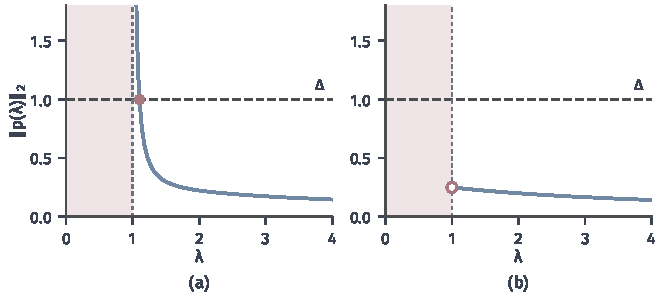
\includegraphics[width=112mm]{figures/05-optimization/02-smooth-optimization/matplotlib/tr-hard-case/figure.pdf}
 \caption{$\bm{B}=\operatorname{diag}(-1,3)$，$\Delta=1$（虚线）时的解长度（蓝）。(a)~$\bm{g}=(0.1,1)^\top$，曲线在$\lambda=1$处趋于无穷，有交点。(b)~$\bm{g}=(0,1)^\top$，曲线只到$1/4$（空心点），与虚线不相交，这是困难情形。}
 \label{fig:tr-hard-case}
\end{BookInlineFigure}

\paragraph{三个不同的量}
子问题的解、模型的下降、真实目标的下降是三件事，下面把它们分开。对候选步$\bm{p}$，定义\term{预测下降}（predicted reduction）和\term{实际下降}（actual reduction）：
\begin{equation}
 \operatorname{pred}(\bm{p})=m(\bm{0})-m(\bm{p}),\qquad
 \operatorname{ared}(\bm{p})=f(\bm{x})-f(\bm{x}+\bm{p}).
 \label{eq:tr-pred-ared}
\end{equation}

子问题的全局解使预测下降最大，却未必使实际下降最大。在原点取$\Delta=2$，全局解是$\bm{p}^\star\approx(-1.988,-0.222)^\top$。由式~\eqref{eq:tr-example-error}，它的模型误差大约是$\tfrac14(1.988)^4\approx3.90$，于是
\[
 \operatorname{pred}(\bm{p}^\star)\approx4.111,\qquad
 \operatorname{ared}(\bm{p}^\star)\approx0.209.
\]

再看同一个球内的另一个点$\bm{p}=(-1.6,-1.2)^\top$。它的预测下降小得多，实际下降反而大一些：
\[
 \operatorname{pred}(\bm{p})=1.92,\qquad
 \operatorname{ared}(\bm{p})\approx0.282.
\]

这个对比说明，模型下降的大小只是在模型的范围内才有意义。图~\ref{fig:tr-three-decreases}画出全局解的两种下降随半径的变化：半径小时两条曲线重合，半径大时预测下降继续上升，实际下降掉头向下。预测和实际的差距正是调整半径的依据，后面第~\ref{sec:tr-acceptance}节用它们的比值组织迭代。

\begin{BookInlineFigure}
 \centering
 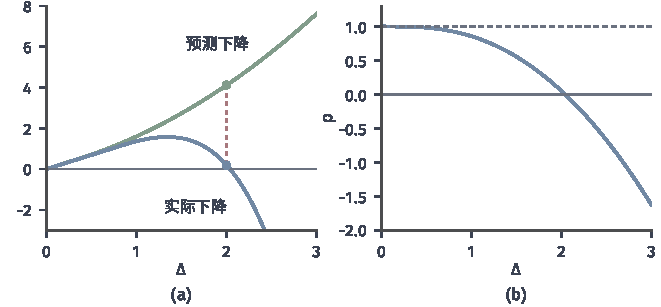
\includegraphics[width=112mm]{figures/05-optimization/02-smooth-optimization/matplotlib/tr-three-decreases/figure.pdf}
 \caption{原点处子问题全局解随半径的变化。(a)~预测下降（绿）与实际下降（蓝），红色虚线标出$\Delta=2$处的差距。(b)~实际下降与预测下降之比$\rho$（蓝），半径越大越偏离$1$，在$\Delta$约为$2$时降到零附近。}
 \label{fig:tr-three-decreases}
\end{BookInlineFigure}
